% !TeX root = RJwrapper.tex
\title{freesurfer: Connecting the Freesurfer Software with R}
\author{by John Muschelli, Elizabeth M. Sweeney, Ciprian M. Crainiceanu}

\maketitle

\abstract{%
We present the package \CRANpkg{freesurfer}, a set of R functions that
interface with Freesurfer, a commonly-used open-source software package
for processing and analyzing structural neuroimaging data. The
\pkg{freesurfer} package performs operations on \code{nifti} image
objects in R using command-line functions from Freesurfer, and returns R
objects back to the user. \pkg{freesurfer} allows users to process
neuroanatomical images and provides functionality to convert and read
the output of the Freesurfer pipelines. We present an example of the
analysis of structural magnetic resonance images, which demonstrates how
R users can interface with Freesurfer and analyze the results of the
complete Freesurfer analysis pipeline.
}

\section{Abstract}\label{abstract}

\begin{Schunk}
\begin{Sinput}
#' if (have_fs()) {
#'    df = aparcs_to_bg(subjects = "bert", measure = "thickness")
#'    print(head(df))
#' }
\end{Sinput}
\end{Schunk}

\begin{Schunk}
\begin{Sinput}
#' if (have_fs()){
#'    img = oro.nifti::nifti(array(rnorm(5*5*5), dim = c(5,5,5)))  
#'    mri_info(img)
#' }


# \dontrun{
#' if (have_fs()){
#'     mri_watershed("/path/to/T1.nii.gz")
#' } 
#' }  

#' @examples \dontrun{
#' if (have_fs()){
#'     mri_normalize("/path/to/T1.nii.gz")
#' } 
#' }

  #' if (have_fs()) {
#'    img = oro.nifti::nifti(array(rnorm(5*5*5), dim = c(5,5,5))) 
#'    res = mri_convert(img, outfile = tempfile(fileext = ".mgz"))
#' } 

  #' if (have_fs()) {
#'    img = oro.nifti::nifti(array(rnorm(5*5*5), dim = c(5,5,5)))  
#'    mnc = nii2mnc(img)
#'    img_file = mnc2nii(mnc)
#' }
#' if (have_fs()) {
#'    img = oro.nifti::nifti(array(rnorm(5*5*5), dim = c(5,5,5)))  
#'    mnc = nii2mnc(img)
#'    img_file = mnc2nii(mnc)
#' }

  #' if (have_fs()) {
#'    img = oro.nifti::nifti(array(rnorm(5*5*5), dim = c(5,5,5)))  
#'    mask = img > 1
#'    res = mri_mask(img, mask)
#' }
#' @examples \dontrun{
#' if (have_fs()){
#'     nu_correct("/path/to/T1.nii.gz")
#' } 
#' } 
\end{Sinput}
\end{Schunk}

\subsection{Introduction}\label{introduction}

\label{sec:intro}

Freesurfer is a commonly-used software for processing and analyzing
anatomical neuroimaging data \citep{fischl2012freesurfer}, developed by
the Laboratory for Computational Neuroimaging at the Athinoula A.
Martinos Center for Biomedical Imaging. This software provides
open-source, command-line tools for image processing tasks such as brain
extraction/skull-stripping \citep{segonne2004hybrid}, bias-field
correction \citep{sled_nonparametric_1998}, segmentation of structures
within the brain \citep{fischl2002whole,fischl2004sequence}, and image
registration \citep{fischl1999high,reuter2010highly}. Many of these
functions are used extensively in medical imaging pipelines and
Freesurfer has a complete pipeline packaged with its software as well.

We have previously published a similar adaptation of the FSL imaging
software \citep{jenkinson_fsl_2012} to R, called \CRANpkg{fslr}
\citep{muschelli2015fslr}. Again, we note that there exist a number of R
packages for reading and manipulating image data, including
\CRANpkg{AnalyzeFMRI} \citep{bordier_temporal_2011}, \CRANpkg{RNiftyReg}
\citep{modat_rniftyreg:_2013}, and \CRANpkg{fmri}
\citep{tabelow_statistical_2011} (see the Medical Imaging CRAN task view
\url{http://cran.r-project.org/web/views/MedicalImaging.html} for more
information). Although these packages are useful for performing image
analysis, much of the fundamental functionality of image preprocessing
and processing that Freesurfer provides are not currently implemented in
R. The \pkg{ANTsR} package (\url{https://github.com/stnava/ANTsR}) has
much of this functionality has been implemented, but this package has
not been released onto CRAN. Moreover, having multiple options for image
processing through R allows for users to compare methods and the
flexibility of using multiple packages to achieve a working data
processing pipeline.

In particular, we provide an interface to users to the state-of-the-art
anatomical processing implemented in Freesurfer, as well as a suite of
tools that simply the analysis of the output of Freesurfer. This will
allow R users to implement complete imaging analysis without necessarily
learning Freesurfer-specific syntax.

\subsection{R imaging objects}\label{r-imaging-objects}

The \CRANpkg{freesurfer} package relies on the \CRANpkg{oro.nifti}
\citep{whitcher_working_2011} package implementation of images (referred
to as \code{nifti} objects) that are in the Neuroimaging Informatics
Technology Initiative (NIfTI) format, as well as other common image
formats such as ANALYZE. Some Freesurfer functions require other
formats, such as MINC
(\url{http://www.bic.mni.mcgill.ca/ServicesSoftware/MINC}). The
Freesurfer installation provides functions to convert from MINC to NIfTI
formats and there are implemented in functions such as \code{nii2mnc}
and \code{mnc2nii} in R. Moreover, the \code{mri\_convert} Freesurfer
function has been interfaced in the \code{freesurfer} package (same
function name), which allows for a more general conversion tool of
imaging types for R users than currently implemented in native R.

\subsection{Reconstruction pipeline in
Freesurfer}\label{reconstruction-pipeline-in-freesurfer}

The Freesurfer pipeline and analysis workflow for neuroanatomical images
is based on a structural magnetic resonance image (MRI) of the brain.
The specific type of image commonly used in this software is a
T1-weighted image, a specific MRI sequence commonly taken. The full
pipeline is implemented in the Freesurfer \code{recon-all} function,
where the ``recon'' stands for reconstruction
(\url{https://surfer.nmr.mgh.harvard.edu/fswiki/recon-all}). Using the
\code{-all} flag in the the \code{recon-all} function performs over 30
different steps and takes 20-40 hours to fully process a subject when
performing all the steps. This process is the common way of fully
processing an T1-weighted image in Freesurfer.

If there are problems with the result of this processing, there are
multiple steps users can edit certain parts of the processing, such as
skull-stripping, where non-brain tissues are removed from the image. The
remainder of the pipeline can be run after these steps. The full
pipeline is broken down into 3 separate steps, referred to as
\code{autorecon1}, \code{autorecon2}, and \code{autorecon3}, which
correspond to the flags in \code{recon-all} used to initiate these
steps. We have written wrapper functions \code{recon\_con1},
\code{recon\_con2}, and \code{recon\_con3}, respectively, for simplicity
to the R user.

\subsection{R function setup}\label{r-function-setup}

To use \pkg{freesurfer}, a working installation of Freesurfer is
required. The following code was run using Freesurfer version
freesurfer-Darwin-lion-stable-pub-v5.3.0. The Freesurfer version can be
accessed using the \code{fs\_version} function. \pkg{freesurfer} must
also have the path of Freesurfer specified. If using R from a shell
environment, and the \code{FREESURFER\_HOME} environment variable is set
(which can be done when installing Freesurfer), \pkg{freesurfer} will
use this as the path to Freesurfer. If using R through a graphical user
interface (GUI) such as RStudio (RStudio, Boston, MA), environmental
variables and paths are not explicitly exported. Therefore,
\code{FREESURFER\_HOME} is not set, \code{freesurfer} will try the
default directories of Mac OSX and Linux. If the user did not perform an
standard installation of Freesurfer, the path to Freesurfer can be
specified using \code{options(freesurfer.path="/path/to/freesurfer")}.

We will discuss the setup functions for the \pkg{freesurfer} package and
how they can be used in analysis and example code. For testing, whether
a user has a Freesurfer installation, the \code{have\_fs} function
provides a logical indicator as a result. The \code{fs\_dir} function
will return the directory of the Freesurfer installation.

\subsubsection{Structure of Freesurfer
analyses}\label{structure-of-freesurfer-analyses}

During the installation of Freesurfer, a series of variables are set up
in the user's shell environment. One of these variables is
\code{SUBJECTS\_DIR}, which refers to a directory of the output of
analysis from all subjects. This setup allows users to simply specify a
subject identifier to analyze, rather than a specific path or multiple
intermediate files.

This setup may not be desirable if the user prefers to structure the
data from multiple studies into different folders. For example, the
\code{asegstats2table} function takes the \textbf{a}natomical
\textbf{seg}mentation \textbf{stat}istics and convert it to a table. The
default argument for \code{asegstats2table} is to pass in a subject name
rather than a file. The \pkg{freesurfer} \code{asegstats2table} function
allows the R user to specify a different subject directory to read in
the file, while not overridding the default set by \code{SUBJECTS\_DIR}.
This functionality allows users to have separate folders with subjects
and read in the data by simply switching the \code{subj\_dir} argument
in the R function.

Similarly to the \code{fs\_dir} function, the \code{fs\_subj\_dir}
function will return the path to the Freesurfer subjects directory if it
is set.

Some Freesurfer functions require an image as an input. For those
functions, the R \pkg{freesurfer} functions that call those Freesurfer
functions will take in a filename or a \code{nifti} object. The R code
will convert the \code{nifti} to the corresponding input required for
Freesurfer. From the user's perspective, the input/output process is all
within R. The advantage of this approach is that the user can read in an
image, do manipulations of the \code{nifti} object using standard syntax
for arrays, and pass this object into the \pkg{freesurfer} R function.
Thus, users can create complete pipelines for the analysis of imaging
data by accessing Freesurfer through \pkg{freesurfer}.

\subsection{Example analyses and use of
functions}\label{example-analyses-and-use-of-functions}

In the default subjects directory in the Freesurfer installation, there
is a subject named ``bert'', where \code{recon-all} was run. In the
sub-directory for subject bert, there are 3 folders which we will
explore the results: ``mri'', which contain imaging data, ``stats'',
whic containing statistics based on structures of the brain, and
``surf'', which contain the surface and curvature output from the
Freesurfer processing.

\subsubsection{Reading in anatomical
statistics}\label{reading-in-anatomical-statistics}

The ``aseg.stats'' in the ``stats'' folder of subject bert corresponds
to measures and statistics from the anatomical segmentation. The
\code{read\_aseg\_stats} function reads this corresponding file and
creates a list of 2 different \code{data.frame}s:

\begin{Schunk}
\begin{Sinput}
file = file.path(fs_subj_dir(), "bert", "stats", "aseg.stats")
out = read_aseg_stats(file)
names(out)
\end{Sinput}
\end{Schunk}

The \code{measures} element corresponds to global measurements of the
brain (e.g.\textasciitilde{}volume of the brain) as well as measures of
gross anatomical structures (e.g.\textasciitilde{}gray matter).

\begin{Schunk}
\begin{Sinput}
head(out$measures[, c("meaning", "value", "units")])
\end{Sinput}
\begin{Soutput}
                                                 meaning          value
1                              brain segmentation volume 1193318.000000
2           brain segmentation volume without ventricles 1174082.000000
3 brain segmentation volume without ventricles from surf 1173867.217735
4            left hemisphere cortical gray matter volume  237947.199463
5           right hemisphere cortical gray matter volume  238312.856735
6                      total cortical gray matter volume  476260.056198
  units
1  mm^3
2  mm^3
3  mm^3
4  mm^3
5  mm^3
6  mm^3
\end{Soutput}
\end{Schunk}

The \code{structures} element corresponds to a set of measures and statistics for a set of fixed anatomical structures.

\begin{Schunk}
\begin{Sinput}
head(out$structures)
\end{Sinput}
\begin{Soutput}
  Index SegId NVoxels Volume_mm3                   StructName normMean
1     1     4    6563     6562.6       Left-Lateral-Ventricle  36.0959
2     2     5     228      228.3            Left-Inf-Lat-Vent  54.8842
3     3     7   15708    15708.2 Left-Cerebellum-White-Matter  92.7562
4     4     8   58536    58535.7       Left-Cerebellum-Cortex  77.2709
5     5    10    8150     8150.4         Left-Thalamus-Proper  92.8386
6     6    11    3214     3213.7                 Left-Caudate  80.9591
  normStdDev normMin normMax normRange
1    12.2771      16      91        75
2    10.7839      22      87        65
3     5.5123      40     107        67
4     9.9521      17     142       125
5     7.0182      49     109        60
6     8.2079      49     105        56
\end{Soutput}
\end{Schunk}

\subsubsection{MRI conversion}\label{mri-conversion}

The typical output format from Freesurfer is MGH/MGZ format, which is
explained here:
\url{https://surfer.nmr.mgh.harvard.edu/fswiki/FsTutorial/MghFormat}. As
NIfTI formats are one of the most common formats and has been the common
format for analysis in the \pkg{oro.nifti} and \pkg{fslr} packages, it
is useful to convert these files to a NIfTI format to use in R. The
\code{mri\_convert} Freesurfer function will be used for that. Here we
will use the T1-weighted image from the ``bert'' subject, convert it to
NIfTI, read it into R, and then plot the image.

\begin{Schunk}
\begin{Sinput}
library(freesurfer)
t1_mgz = file.path(fs_subj_dir(), "bert", "mri", "T1.mgz")
t1_nii_fname = tempfile(fileext = ".nii.gz")
freesurfer::mri_convert(t1_mgz, t1_nii_fname)
library(fslr)
img = fslr::readnii(t1_nii_fname)
fslr::ortho2(img)
\end{Sinput}

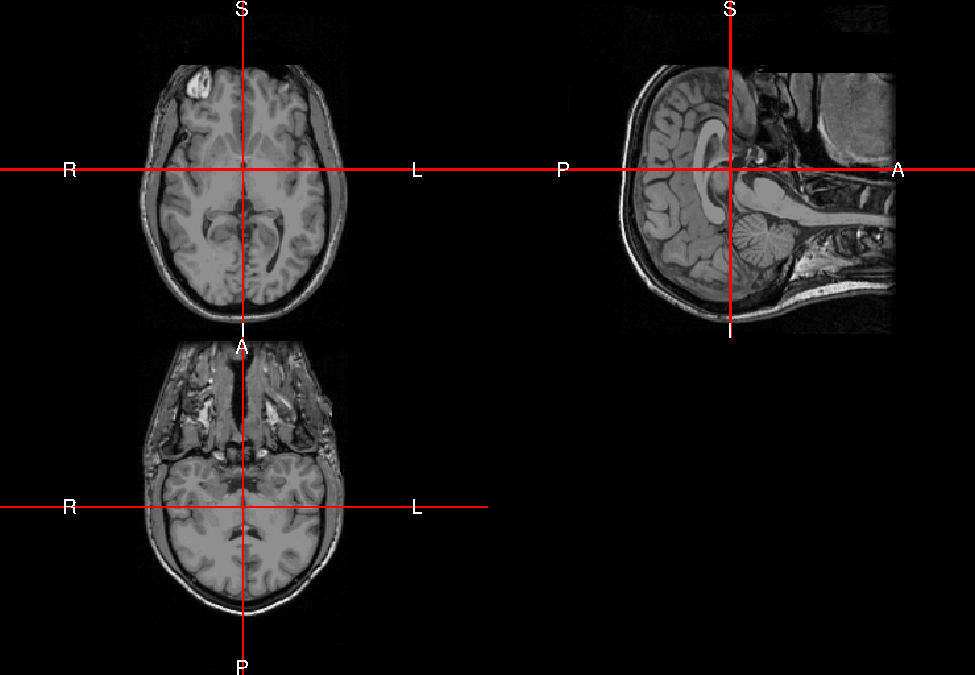
\includegraphics{Freesurfer_files/figure-latex/mri_convert-1} \end{Schunk}

\subsection{Brain extraction}\label{brain-extraction}

The \code{mri\_watershed} function will segment the brain from the rest
of the image. We ca pass in the \code{nifti} object and the output is a
brain-extracted \code{nifti} object.

\begin{Schunk}
\begin{Sinput}
ss = mri_watershed(img)
ortho2(ss)
\end{Sinput}

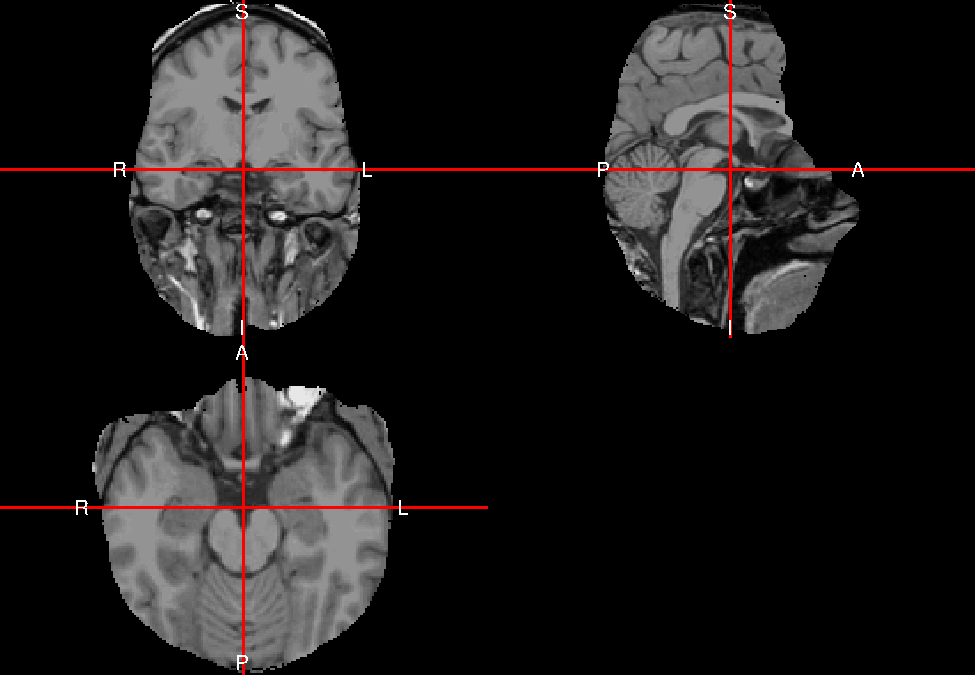
\includegraphics{Freesurfer_files/figure-latex/watershed-1} \end{Schunk}

As the result in a \code{nifti} object, we can create a mask by standard
logical operations:

\begin{Schunk}
\begin{Sinput}
mask = ss > 0
\end{Sinput}
\end{Schunk}

\subsection{Bias-field correction}

MRI images typically exhibit good contrast between soft tissue classes,
but intensity inhomogeneities in the radio frequency field can cause
differences in the ranges of tissue types at different spatial locations
(e.g.\textasciitilde{}top versus bottom of the brain) . These
inhomogeneities/non-uniformities can cause problems with algorithms
based on histograms, quantiles, or raw intensities
\citep{zhang_segmentation_2001}. Therefore, correction for image
inhomogeneities is a crucial step in many analyses. The Freesurfer
function \code{nu\_correct} performs the non-uniformity correction by
\citet{sled_nonparametric_1998} and the \pkg{freesurfer} function of the
same name will run the correction and return an image.

The Freesurfer \code{nu\_correct} function requires a MNC format
(\url{http://www.bic.mni.mcgill.ca/ServicesSoftware/MINC}). For this to
work, you can convert the \code{nifti} object to a MNC file using
\code{nii2mnc} and pass that file into \code{nu\_correct}. The
\pkg{freesurfer} \code{nu\_correct} function will run the correction and
then convert the output MNC to a NIfTI object.

\begin{Schunk}
\begin{Sinput}
mnc = nii2mnc(img)
print(mnc)
nu_from_mnc = nu_correct(file = mnc)
class(nu_from_mnc)
ortho2(nu_from_mnc)
\end{Sinput}

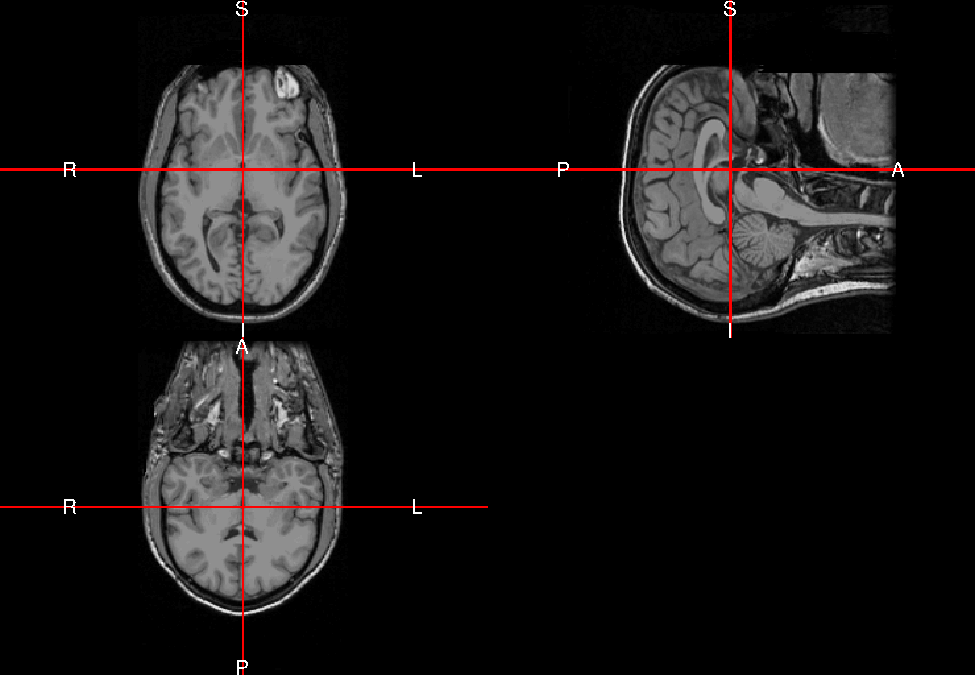
\includegraphics{Freesurfer_files/figure-latex/nu_correct_mcn2nii-1} \end{Schunk}

You can also pass in a \code{nifti} object in directly, and the
\pkg{freesurfer} \code{nu\_correct} function will automatically convert
any NIfTI input files, and then run the correction. We can also pass in
a mask (generated from above) to run the correction only the areas of
the brain.

\begin{Schunk}
\begin{Sinput}
nu_nifti = nu_correct(file = img, mask = mask)
class(nu_from_mnc)
\end{Sinput}
\end{Schunk}

\subsection{Image preprocessing with \pkg{fslr}}

We present a complete analysis of structural magnetic resonance imaging
(MRI) data performed using \pkg{fslr} and R. Images were obtained from a
patient with multiple sclerosis (MS) at 2 different visits
\citep{sweeney_automatic_2013}, located at \url{bit.ly/FSL_Data}. At
each visit, the image modalities obtained were T1-weighted (T1),
T2-weighted (T2), fluid-attenuated inversion recovery (FLAIR), and
proton density (PD). In this example we will perform a MRI bias-field
correction using FAST (FMRIB's Automated Segmentation Tool)
\citep{zhang_segmentation_2001}, co-register scans within visits to the
T1 image of that visit, and register T1 images between visits. Once
these operations have been performed, one can take within-modality
difference images to see the changes between visits. We will also
register all images to a common stereotaxic template, as this is common
in population-based analyses.

\subsection{Section title in sentence
case}\label{section-title-in-sentence-case}

This section may contain a figure such as Figure \ref{figure:rlogo}.

\begin{figure}[htbp]
  \centering
  
\includegraphics{Rlogo}
  \caption{The logo of R.}
  \label{figure:rlogo}
\end{figure}

\subsection{Another section}\label{another-section}

There will likely be several sections, perhaps including code snippets,
such as:

\begin{Schunk}
\begin{Sinput}
x <- 1:10
x
\end{Sinput}
\end{Schunk}

\subsection{Conclusion}\label{conclusion}

The neuroimaging community has developed a large collection of tools for
image processing and analysis. R has a number of packages to perform
operations on images; \BIOpkg{EBImage} is one good example
\citep{EBImage}. Much of the fundamental functionality of neuroimage
processing is not currently available in R, such as brain extraction and
tissue segmentation. We present \pkg{fslr} to provide R users functions
for image processing and analysis that are based on FSL, an established
image processing and analysis software suite. Interfacing R with
existing, powerful software provides users with thoroughly-tested
software and an additional community of users, which would not be
available if the functions were rewritten in R. \pkg{fslr} should be
easy to use for any standard R user; the workflow allows R users to
manipulate array-like \code{nifti} objects, pass them to \pkg{fslr}
functions, which return \code{nifti} objects. Moreover, as FSL and R are
open source and free, this software is readily available to all users.

There has been an increasing popularity of similar interfacing of tools
within the Python community such as Nipype
\citep{gorgolewski_nipype:_2011}
(\url{https://qa.debian.org/popcon.php?package=nipype}). As many users
of R may not have experience with Python or bash scripting, we believe
\pkg{fslr} provides a lower threshold for use in the R community. Other
packages provide R users additional neuroimaging processing
functionality such as \CRANpkg{AnalyzeFMRI}
\citep{bordier_temporal_2011}, \CRANpkg{RNiftyReg}
\citep{modat_rniftyreg:_2013}, and \CRANpkg{fmri}
\citep{tabelow_statistical_2011}.

For example, other inhomogeneity correction methods exist, such as the
popular N3 \citep{sled_nonparametric_1998} and N4
\citep{tustison_n4itk:_2010}, methods which are not implemented in
\pkg{fslr}. \pkg{ANTsR} (\url{http://stnava.github.io/ANTsR/index.html})
is a currently unpublished R package that interfaces with the ANTs
(advanced normalization tools) software suite
\citep{avants_reproducible_2011}. ANTs has implementations of these
correction methods, an increased set of registration techniques, and
other methods for image processing. Other packages such as this, along
with \pkg{fslr}, can create a diverse set of tools for neuroimaging
within R, building on preexisting and widely-accepted software.

Most importantly, as \pkg{fslr} is based on the R framework, all the
benefits of using R are available, such as dynamic documents,
reproducible reports, customized figures, and state-of-the-art
statistical methods. These benefits provide unique functionality
compared to other software packages for neuroimaging.

All data and code processed here is located at
\url{https://github.com/muschellij2/FSLR_Data}.

\subsection{Summary}\label{summary}

This file is only a basic article template. For full details of
\emph{The R Journal} style and information on how to prepare your
article for submission, see the
\href{https://journal.r-project.org/share/author-guide.pdf}{Instructions
for Authors}. \bibliography{RJreferences}

\address{%
John Muschelli\\
Johns Hopkins Bloomberg School of Public Health\\
Department of Biostatistics\\ 615 N Wolfe St, Baltimore, MD, 21205\\
}
\href{mailto:jmuschel@jhsph.edu}{\nolinkurl{jmuschel@jhsph.edu}}

\address{%
Elizabeth M. Sweeney\\
Rice University\\
Department of Statistics\\ 6100 Main St, Duncan Hall, Houston, TX, 77005\\
}
\href{mailto:ems15@rice.edu}{\nolinkurl{ems15@rice.edu}}

\address{%
Ciprian M. Crainiceanu\\
Johns Hopkins Bloomberg School of Public Health\\
Department of Biostatistics\\ 615 N Wolfe St, Baltimore, MD, 21205\\
}
\href{mailto:ccraini1@jhu.edu}{\nolinkurl{ccraini1@jhu.edu}}

